\documentclass{beamer}

\usetheme{Antibes}

%\usetheme{split}
%\usetheme{Madrid}
%\usetheme{Berkeley}
\usecolortheme[RGB={120,0,0}]{structure}
\setbeamertemplate{blocks}[rounded][shadow=true]
\setbeamertemplate{footline}{\hfill\insertframenumber{}/\inserttotalframenumber\hspace*{0.02cm}}
\usepackage[utf8]{inputenc}   % pacote para acentuao
\usepackage{graphicx}
\usepackage{subcaption}

%\usepackage[latin1]{inputenc}

\beamertemplateballitem
\beamertemplatenavigationsymbolsempty

\begin{document}

\title{Container technologies on HPC applications}
\author{\large Guilherme Rezende Alles\\
\footnotesize CPM270 - Introduction to High Performance Computing\\
\small
\vspace*{1.5cm}
Instituto de Informática\\
Universidade Federal do Rio Grande do Sul
}
\logo{
\includegraphics[scale=0.3]{inf}}
\date{21 de Junho de 2018}
\frame{\titlepage}
\frame{\frametitle{Roteiro}\tableofcontents[hideallsubsections]}


\section{Introdução}
\frame{\tableofcontents[currentsection,hideothersubsections]}
\subsection{Motivação}
\frame{\frametitle{Motivação}
    \begin{itemize}
        \item Virtualização permite redução de custos de infraestrutura
        \begin{itemize}
            \item Desvantagem: impacto no desempenho de aplicações
            \item Opção: virtualização em nível de SO (contêineres)
        \end{itemize}
    \end{itemize}
    \begin{itemize}
        \item Popularidade de contêineres na indústria de software
        \begin{itemize}
            \item Todos os serviços da Google executam em contêineres
        \end{itemize}
    \end{itemize}
    \begin{itemize}
        \item Vantagens relevantes em computação científica
        \begin{itemize}
            \item Reprodutibilidade de experimentos
            \item Portabilidade (\textit{Bring Your Own Environment})
        \end{itemize}
    \end{itemize}
}

\subsection{Objetivos}
\frame{\frametitle{Objetivos}
    \begin{itemize}
        \item Avaliar a viabilidade de contêineres no contexto de aplicações paralelas
        \begin{itemize}
            \item Compatibilidade dessa solução com ambientes HPC
            \item Impacto no desempenho
        \end{itemize}
    \end{itemize}
    \vspace*{0.5cm}
    \begin{itemize}
        \item Comparar duas tecnologias de contêineres ao desempenho nativo
        \begin{itemize}
            \item Docker e Singularity
        \end{itemize}
    \end{itemize}
}

\section{Fundamentação teórica}
\frame{\tableofcontents[currentsection,hideothersubsections]}
\subsection{Contêineres}
\frame{\frametitle{Contêineres}
    \begin{itemize}
        \item Ambiente de execução virtualizado
        \item Objetivos principais
        \begin{itemize}
            \item Isolamento de processos
            \item Encapsulamento de dependências
        \end{itemize}
        \item Restrito a sistemas operacionais GNU/Linux 
        \begin{itemize}
            \item \textit{Kernel} é compartilhado entre contêineres e sistema nativo
        \end{itemize}
    \end{itemize}
    \begin{figure}
        \centering
        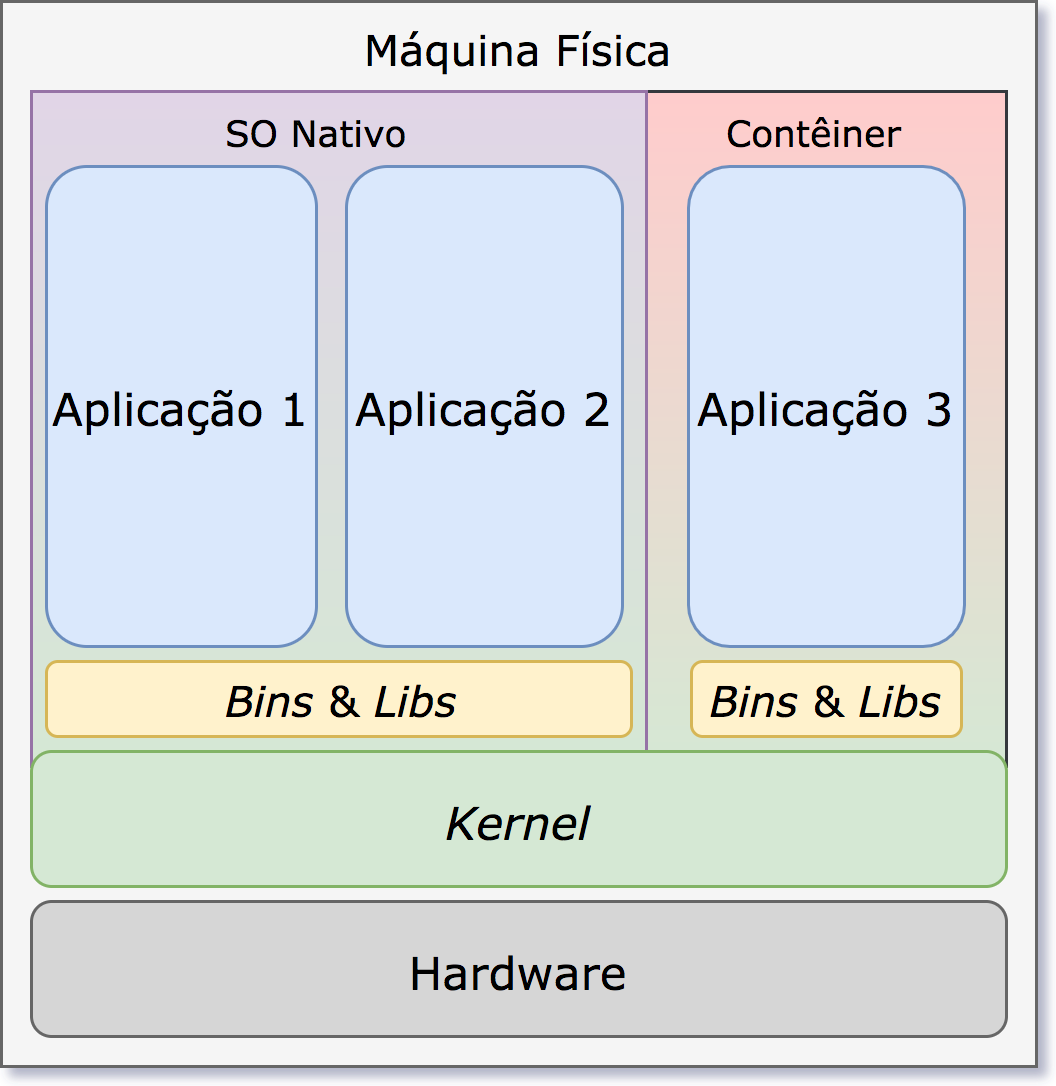
\includegraphics[width=.375\textwidth]{conteineres.png}
    \end{figure}
}

\section{Tecnologias de contêineres}
\frame{\tableofcontents[currentsection,hideothersubsections]}

\subsection{Docker}
\frame{\frametitle{Docker}
    \begin{figure}
        \centering
        \vspace*{-1cm}
        
\includegraphics[width=.3\textwidth]{docker-logo.png}
        \vspace*{-0.25cm}
    \end{figure}
    \begin{itemize}
        \item Plataforma de contêineres mais popular na indústria de software
    \end{itemize}
    \begin{itemize}
        \item Usa a API de \textit{namespaces} para isolamento completo
        \begin{itemize}
            \item Processos têm a impressão de estarem executando em uma máquina dedicada
        \end{itemize}
    \end{itemize}
    \begin{itemize}
        \item \textit{Docker daemon} executa como \textit{root}
        \begin{itemize}
            \item Segurança comprometida em ambientes compartilhados
        \end{itemize}
    \end{itemize}
}

\frame{\frametitle{Implementação de \textit{cluster} com Docker}
    \begin{itemize}
        \item Virtualização da camada de rede
        \begin{itemize}
            \item Interface virtual conecta contêineres em uma única máquina
            \item Para múltiplas máquinas físicas, é necessária uma rede virtual
        \end{itemize}
    \end{itemize}
    \begin{itemize}
        \item \textit{Docker Swarm}
        \begin{itemize}
            \item Configura múltiplas máquinas físicas em um \textit{cluster}, conectado por uma rede de sobreposição
            \item Contêineres são distribuídos múltiplas máquinas físicas
        \end{itemize}
    \end{itemize}
    \begin{figure}
        \centering
        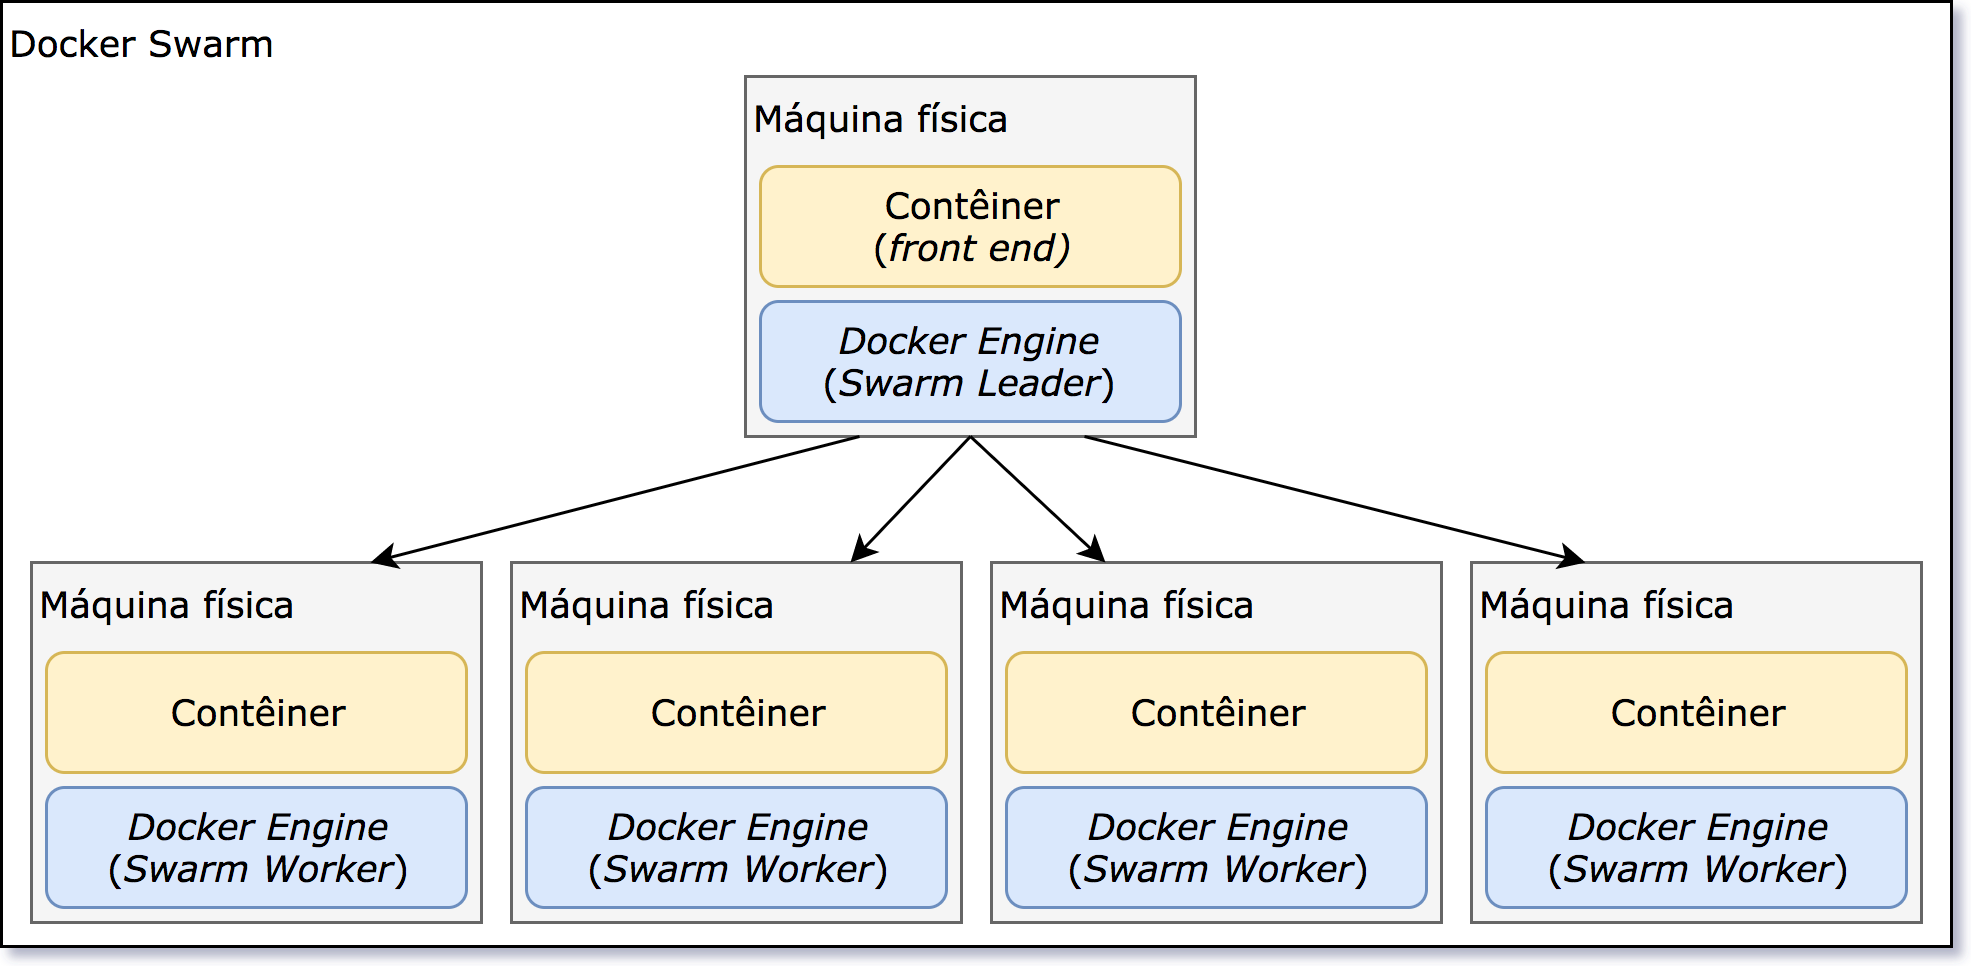
\includegraphics[width=.6\textwidth]{swarm-cluster.png}
    \end{figure}
}

\subsection{Singularity}
\frame{\frametitle{Singularity}
    \begin{figure}
        \centering
        \vspace*{-1cm}
        
\includegraphics[width=.1\textwidth]{singularity-logo.png}
        \vspace{-0.5cm}
    \end{figure}
    \begin{itemize}
        \item Desenvolvido para uso com aplicações de alto desempenho
        \item Principais objetivos
        \begin{itemize}
            \item Reprodutibilidade
            \item Portabilidade
            \item Integração nativa com recursos comuns em \textit{clusters}
        \end{itemize}
        \vspace*{0.2cm}
        \item Nível de virtualização menos invasivo
        \begin{itemize}
            \item Contêiner é visto como um processo do usuário no sistema nativo
        \end{itemize}
    \end{itemize}
}

\frame{\frametitle{Execução do Singularity em um cluster}
    Singularity permite integração nativa com ferramentas instaladas, por conta do modelo de virtualização menos invasivo
    \vspace*{0.3cm}
    \begin{itemize}
        \item Contêineres são processos visíveis no sistema nativo
        \begin{itemize}
            \item Rede, IPC e usuários são compartilhados
        \end{itemize}
        \vspace*{0.3cm}
        \item Integração trivial com escalonadores de tarefas (como, por exemplo, SLURM ou \textit{mpirun})
        \begin{itemize}
            \item No sistema nativo: \textit{mpirun -np 4 ./container.img}
        \end{itemize}
        \vspace*{0.3cm}
    \end{itemize}
}

\section{Avaliação experimental}
\frame{\tableofcontents[currentsection,hideothersubsections]}

\subsection{Recursos utilizados}
\frame{\frametitle{Plataforma de hardware}
    \begin{itemize}
        \item Grid5000
        \begin{itemize}
            \item Plataforma para experimentos em computação
            \item Segue uma infraestrutura do tipo \textit{grid}
        \end{itemize}
    \end{itemize}
    \vspace*{-0.2cm}
    \begin{figure}
        \centering
        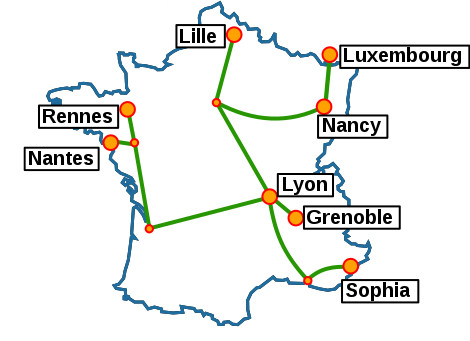
\includegraphics[width=.3\textwidth]{grid5000.png}
    \end{figure}
    \vspace*{-0.2cm}
    \begin{itemize}
        \item Testes experimentais na \textit{Grid5000}
        \begin{itemize}
            \item Até 5 nodos do \textit{cluster} \textit{Graphene}, no \textit{site} \textit{Nancy}
            \begin{itemize}
                \item Intel Xeon X3340 (4 \textit{cores}, 2.53GHz)
                \item 16GB DDR3 RAM
                \item Gigabit Ethernet
            \end{itemize}
        \end{itemize}
    \end{itemize}
}

\frame{\frametitle{Ambiente de software}
    \begin{itemize}
        \item Sistema operacional
        \begin{itemize}
            \item Linux, distribuição Debian 9
            \begin{itemize}
                \item Melhor compatibiliade com a Grid5000
            \end{itemize}
            \item MPICH 3.2
            \item OpenMP 4.5
        \end{itemize}
        \vspace*{0.2cm}
        \item Benchmarks:
        \begin{itemize}
            \item Ondes3D (MPI + OpenMP)
            \begin{itemize}
                \item Desbalanceamento de carga, comunicação frequente
            \end{itemize}
            \item Ping-Pong (MPI)
            \begin{itemize}
                \item Desempenho da rede
            \end{itemize}
            \item NAS Parallel Benchmarks - EP (MPI)
            \begin{itemize}
                \item Baixa comunicação, altamente paralelizável
            \end{itemize}
        \end{itemize}
    \end{itemize}
}

\subsection{Resultados}
\frame{\frametitle{\textit{Benchmark} Ondes3D - 50 timesteps}
    \vspace*{-0.2cm}
    \begin{figure}
        \centering
        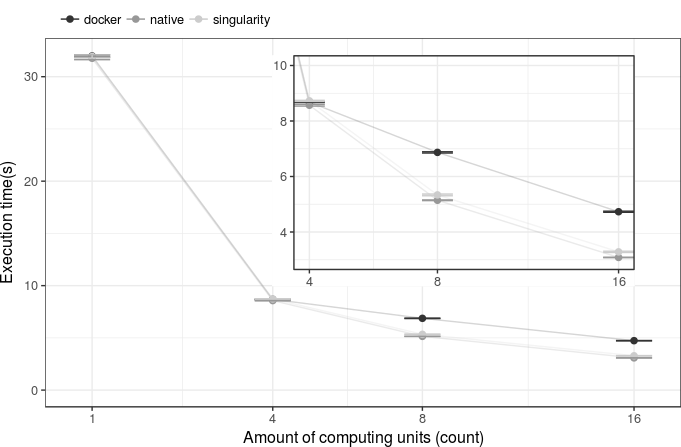
\includegraphics[width=.75\textwidth]{ondes3d-essai-50ts.png}
    \end{figure}
    \begin{itemize}
        \item Docker apresenta desempenho pior
        \begin{itemize}
            \item Sobrecusto da rede virtual
        \end{itemize}
        \item Singularity apresenta resultados próximos do nativo
    \end{itemize}
}

\frame{\frametitle{\textit{Benchmark} Ping-Pong}
    \begin{figure}
        \centering
        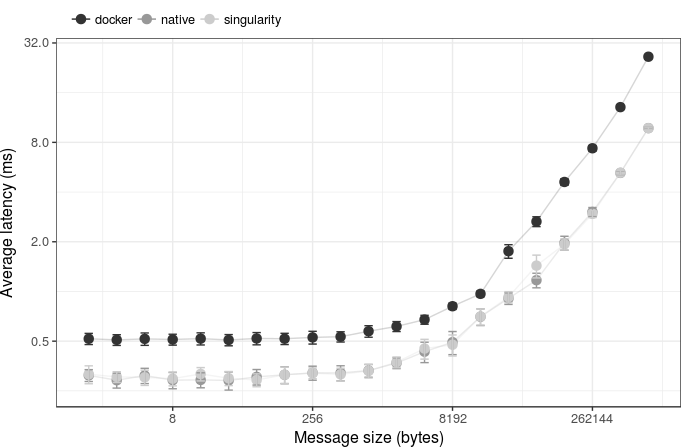
\includegraphics[width=0.7\textwidth]{ping-pong.png}
    \end{figure}
    \begin{itemize}
        \item Evidencia a o \textit{overhead} na rede virtualizada
    \end{itemize}
}

\frame{\frametitle{\textit{Benchmark} NAS EP - Categoria B}
    \begin{figure}
        \centering
        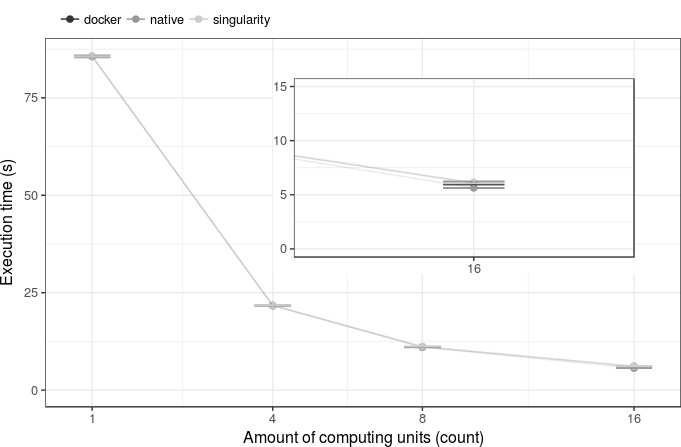
\includegraphics[width=0.8\textwidth]{ep-b.png}
    \end{figure}
    \begin{itemize}
        \item Desempenho do Docker e Singularity é comparável
        \item Uso de contêineres não degrada o desempenho nativo
    \end{itemize}
}

\frame{\frametitle{\textit{Benchmark} NAS EP - Categoria B, Alpine Linux}
    \begin{figure}
        \centering
        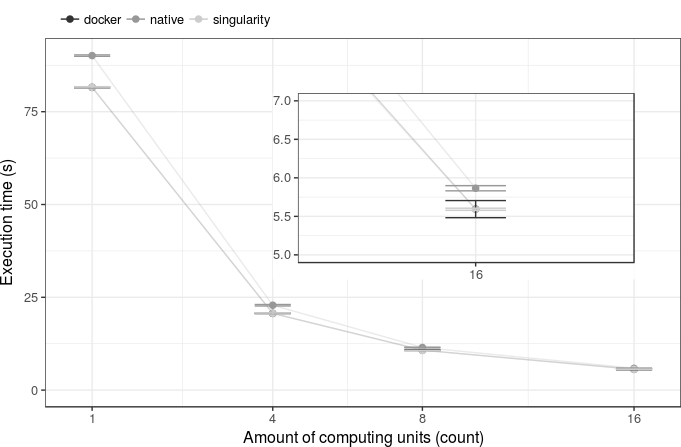
\includegraphics[width=0.8\textwidth]{ep-b-alpine.png}
    \end{figure}
    \begin{itemize}
        \item É possível modificar facilmente o ambiente de execução
        \item Uso de bibliotecas diferentes pode melhorar o desempenho
    \end{itemize}
}

\section{Conclusões}
\frame{\tableofcontents[currentsection,hideothersubsections]}

\subsection{}
\frame{\frametitle{Conclusões}
    \begin{itemize}
        \item Contêineres são uma plataforma viável para virtualização de aplicações HPC
        \begin{itemize}
            \item Baixo sobrecusto computacional (\textit{overhead})
            \item Auxilia a reprodutibilidade de experimentos
            \item Permite maior flexibilidade do ambiente de execução
        \end{itemize}
        \vspace*{0.5cm}
        \item Na tecnologia atual, contêineres Singularity são mais apropriados para ambientes de HPC
        \begin{itemize}
            \item Rede nativa
            \item Usuário sem privilégios adicionais
            \item Integração nativa com ferramentas comuns
        \end{itemize}
    \end{itemize}
}

\subsection{}
\frame{
    \frametitle{Obrigado!}
    \centering
    Guilherme Rezende Alles - gralles@inf.ufrgs.br\\
    \vspace*{1cm}
    \textbf{Perguntas?}\\
    \vspace*{0.5cm}
    
\includegraphics[scale=0.55]{inf} \hspace{1cm}
    
\includegraphics[scale=0.13]{ufrgs.png}
}


\end{document}




